\chapter{Funktionalität}
\textcolor{red}{Funktionalität: Spezifikation der einzelnen Produktfunktionen mit genauer und detaillierter Beschreibung.}

Zur Entkopplung einzelner Module und leichteren Wartbarkeit verwendet die Anwendung eine Drei-Schichten Architektur bestehend aus Nutzeroberfläche, Business-Schicht und Daten-Schicht. 
\begin{figure}[h]
\begin{center}
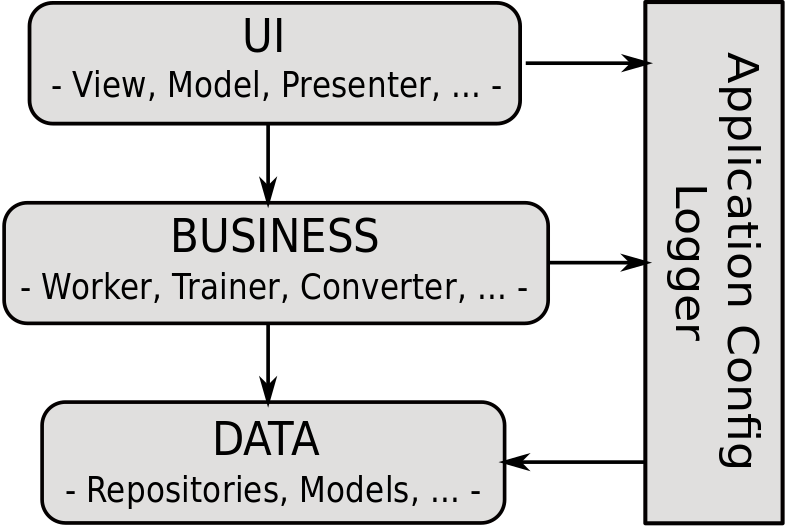
\includegraphics[width=10cm]{Abbildungen/UML/jan/SchichtenModell.png}
\end{center}
\end{figure}
Die Nutzeroberfläche dient der Nutzerinteraktion sowie der Darstellung der Eingabe- sowie verarbeiteten Daten. Sie implementiert dabei das MVP-Muster...

\textcolor{red}{ @Daniel: Hier bitte dein Part für das MVP-Pattern rein!!!}


In der Buisiness-Schicht werden alle fachspezifischen Verarbeitungen vorgenommen. Hierunter fallen beispielsweise die Vorwärtsberechnung sowie das Training eines künstlichen neuronalen Netzes oder die Konvertierung von Daten. Dazu werden für jede Entität spezifizsche Worker-Klassen zur Verfügung gestellt, die diese Aufgaben durchführen können.

\begin{figure}[h]
\begin{center}
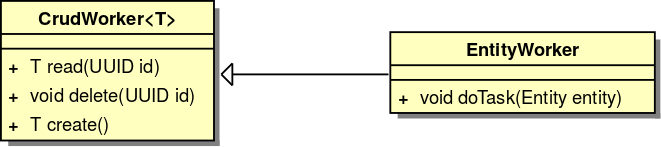
\includegraphics[width=10cm]{Abbildungen/UML/jan/workerClassDiagramm.png}
\end{center}
\end{figure}

Als unterste Schicht der Anwendung dient die Daten-Schicht der Persistierung von Daten. Hierfür stehen ihr diverse, von CRUD-Worker angesprochene Repositories zur Verfügung, die je nach Bedarf Daten (hier im Wesentlichen das Neuronale Netz) in eine Datenbank oder externe Dateien schreiben können.

In den nächsten Unterabschnitten folgt die ausführliche Beschreibung und geplante Umsetzung der von der Anwendung zu erbringenden Funktionalitäten.  


\begin{itemize}
  \item Typische Arbeitsabläufe
  \item Keine Angabe von typischen Verwaltungsfunktionen (CRUD \footnote{Create,
Read, Update, Delete}
\end{itemize}


\section{Training eines Neuronalen Netzes}
